Coaxial cables are the gold standard cable for transmitting electrical signals. First invented for telegraph transmission in 1880 
%as patent number 1407 (1,800,000 patients are filed per year now) 
by Oliver Heaviside, it has since been used for mass deployment of our major information age, specifically used for television and the internet. However it is also in every lab since it is can carry signals with the highest accuracy, but the coaxial cable also has inbuilt characteristics which significantly affect the signals as they propagate so the purpose of this experiment is to explore and measure some of these characteristics.\\

A coaxial cable is named as such because it has layers of conductors throughout its axis. There are four distinct layers: the center is a conductive wire, then a dielectric layer around it, followed by another conductive layer, and finally a insulating layer for protection. These layers can be seen in a cross-section of a wire as shown in Figure \ref{fig:Cable}.

\begin{figure}[H]
\centering
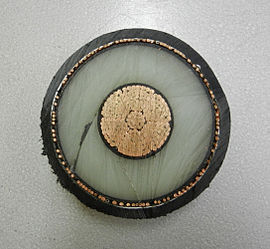
\includegraphics[width=0.25\textwidth]{figures/Coaxial_cable.jpg}
\caption{Coaxial cable cross-section demonstrating the four layers \cite{pict_cable}. }
\label{fig:Cable}
\end{figure}

Generally, alternating current (AC) electricity is transmitted through the cables, so it is important to consider the characteristics of these AC waves as the propagate through the wave-guide, as well as measure and derive characteristics of each cable.\\

In this paper we will first explore the theory of a coaxial cable as a wave-guide, and then experimentally measure several properties of the cable. They are the: relative permittivity of the dielectric, speed of electrical transmission, capacitance, inductance, impedance. We observe other trends that are seen in the cable mainly due to cable terminations.